\chapter{Código intermedio de GCC}

A continuación se exponen los distintos códigos intermedios que GCC utiliza en la compilación. 
Los distintos códigos intermedios están relacionados en la forma que la salida 
de cada uno es la entrada del siguiente, avanzando desde una representación general de alto nivel 
hacia una específica de bajo nivel. 

\begin{figure}[ht]
    \begingroup
        \centering
            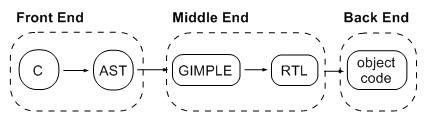
\includegraphics[width=1\textwidth,height=1\textheight,keepaspectratio]{gcc_process}
            \caption{Proceso de compilación de GCC.}
            \label{fig:gcc_process}
        \par
    \endgroup
\end{figure}

\section{Analizador léxico y sintáctico}
El analizador léxico lee la secuencia de caracteres desde la salida del preprocesador y agrupa los 
caracteres en secuencias llamadas lexemas.
Por cada lexema, el analizador genera un token con la manera:
\begin{center}
    [\emph{token name, attribute value}]
\end{center}
Donde \emph{token name} son símbolos abstractos usados durante el análisis sintáctico,
y \emph{attribute value} es un puntero a una entrada en la tabla de símbolos.
GCC no permite obtener los \emph{tokens} válidos en forma de texto. Es un archivo interno.
El analizador sintáctico chequea si la gramática del lenguaje acepta la secuencia
de \emph{tokens} generados por el analizador léxico, si no reporta errores de sintaxis. 
Además, el analizador sintáctico utiliza el primer componente de cada token para crear una representación en manera de árbol 
que muestre la estructura de los \emph{tokens}, es decir, un árbol sintáctico\cite{GCCast}.
Con el \emph{flag} -fdump-tree-original-raw se obtiene la representación textual del árbol abstracto sintáctico.

\begin{lstlisting}[label=comandoC, caption= Comando de compilación para obtener codigo-ejemplo.c.005t.original \cite{repositorio} para GCC., language=bash]
    $ gcc -fdump-tree-original-raw codigo-ejemplo.c -o codigo-ejemplo  \end{lstlisting}

\section{Analizador semántico}
El analizador semántico utiliza el árbol sintáctico y la información de la tabla de símbolos 
para revisar la consistencia semántica del programa fuente con respecto a la definición del lenguaje. 

\section{\emph{Generic}}

\emph{Generic} es un código intermedio independiente del lenguaje con estructura de árbol 
que es generado por el \emph{front end}. \emph{Generic} es capaz de representar todos los 
lenguajes admitidos por GCC. \emph{Generic} se produce eliminando construcciones específicas 
del lenguaje del árbol de parseo. 
GCC pasa del árbol abstracto sintáctico a la representación en \emph{Gimple} en lenguajes como C.

\section{\emph{Gimple}}

\emph{Gimple} es un código intermedio de tres direcciones resultante de desglosar \emph{Generic} en tuplas 
de no más de tres operandos, a través de la herramienta interna de GCC llamada \emph{Gimplifier}. 
\emph{Gimple} introduce variables temporales para poder computar expresiones complejas y permite 
supervisar el flujo de control a nivel inferior con sentencias secuenciales y saltos incondicionales. 
\emph{Gimple} es el código intermedio principal de GCC (los lenguajes C y C++ se convierten a \emph{Gimple} 
sin pasar por \emph{Generic}), ademas de ser conveniente para optimizar. 

Existen tres tipos de \emph{Gimple}:

\begin{itemize}
    \item \emph{Gimple} de alto nivel que es lo que se obtiene después de desglosar el \emph{Generic}.
    \item \emph{Gimple} de bajo nivel que se obtiene al linealizar todas las estructuras de flujo de control de 
            del \emph{Gimple} de alto nivel, incluidas las funciones anidadas, el manejo de excepciones y los bucles.
    \item \emph{Gimple} SSA es el \emph{Gimple} de bajo nivel reescrito en la forma SSA\cite{GCCintermediate}.
\end{itemize}

Con el \emph{flag} -fdump-tree-gimple se obtiene la representación en la forma de \emph{Gimple}.

\begin{lstlisting}[label=comandoC, caption= Comando de compilación para obtener codigo-ejemplo.c.006t.gimple \cite{repositorio} para GCC., language=bash]
    $ gcc -fdump-tree-gimple codigo-ejemplo.c -o codigo-ejemplo  \end{lstlisting}

Además, con el \emph{flag} -fdump-tree-all-graph GCC genera muchos archivos con la extension .cfg 
los cuales pueden visualizarse con una herramienta online Graphviz \cite{GraphvizOnline}. Esta herramienta permite 
ver la evolución del código en las distintas pasadas de una manera mucho más conveniente 
para el usuario. 

\begin{lstlisting}[label=comandoC, caption= Comando de compilación del archivo codigo-ejemplo.c \cite{repositorio} para GCC., language=bash]
    $ gcc -fdump-tree-all-graph codigo-ejemplo.c -o codigo-ejemplo  \end{lstlisting}


\section{\emph{Register Transfer Language}}

\emph{Register Transfer Language} es un código intermedio de bajo nivel semejante al lenguaje ensamblador.
La mayor parte del trabajo del compilador se realiza en \emph{Register Transfer Language}. Tiene una forma interna, 
formada por estructuras que apuntan a otras estructuras, y una forma textual 
que se utiliza en la descripción de la máquina y en los volcados de depuración 
impresos. El formulario textual usa paréntesis anidados para indicar los punteros en el formulario interno.
Con el \emph{flag} -fdump-rtl-final se obtiene la representación en la forma de \emph{Register Transfer Language} ya optimizado por el compilador.

\begin{lstlisting}[label=comandoC, caption= Comando de compilación para obtener codigo-ejemplo.c.330r.final \cite{repositorio} para GCC., language=bash]
    $ gcc -fdump-rtl-final codigo-ejemplo.c -o codigo-ejemplo  \end{lstlisting}

\section{\emph{Assembler}}
Por último, es posible obtener la salida en \emph{Assembler} con el \emph{flag} -S.

\begin{lstlisting}[label=comandoC, caption= Comando de compilación para obtener codigo-ejemplo.s \cite{repositorio} para GCC., language=bash]
    $ gcc -S codigo-ejemplo.c -o codigo-ejemplo.s  \end{lstlisting}



